\chapter{System Architecture}


\section{Server to Server}

\begin{figure}[hb]
\centering
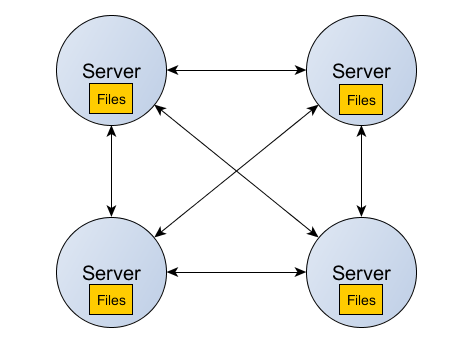
\includegraphics[scale=0.5]{images/architechure-diagram-server-server.png}
\caption{The highest level server-to-server system architecture}
\end{figure}

Figure 6.1 details the overall, top-level view of our P2P network.  Our system is composed of a geographically distributed network of servers.  Each user or corporation which uses to use our network purchases one of these servers to place on their own LAN.  These servers work together to distribute and share data which has been backed up.  Even if one or multiple of the servers goes down, the data should be preserved due to the storage redundancy.

\clearpage


\section{Server to Client}

\begin{figure}[hb]
\centering
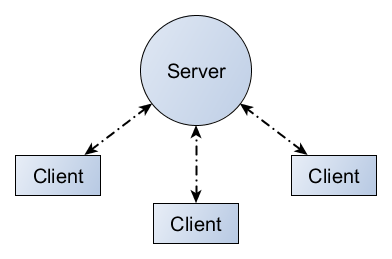
\includegraphics[scale=0.5]{images/architechure-diagram-server-client3.png}
\caption{The highest level server-to-server system architecture}
\end{figure}

Figure 6.2 zooms in on a single server, with each of its own individual client connections. Each computer will start an OpenSSH server on boot. This, with the appropriate firewall settings, will allow the storage device to contact the computer and access its files. The storage device is made aware of the clients through a packet broadcast by the client during setup. Once that initiation is complete the backup server can connect to each client and download each file, block-wise.


\clearpage


\section{Server Architecture}

\begin{figure}[hb]
\centering
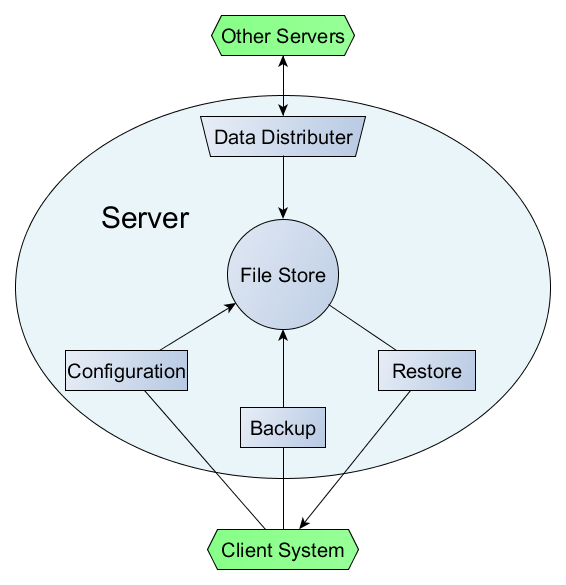
\includegraphics[scale=0.5]{images/architechure-diagram2.png}
\caption{A View of the Data Flow Through our Server}
\end{figure}

 Figure 6.3 details the internal structure of each individaul server, which a user purchases to place on their own LAN.  We see that each server has a connection into the larger P2P network of servers.  Also, each server connects to client machines on its LAN.  When a backup is initiated, either manually by a user or automatically according to scheduling, the Backup application on the server can start to retreive blocks of data from the client using OpenSSH.  Each block is stored in a document-oriented File Store and stored in a document along with its hash. Documents associating files with a set of hashes and grouping files with directories are stored in separate documents. Each computer is represented by a document that specifies the files in that computer that are backed up in addition to that computer's scheduling configuration. Once the data and its form has been successfully stored, the Data Distributer is responsible for finding other storage devices and replicating the data to each device.  When a user wishes to make changes of configuration, such as scheduling backup times or choosing which files to be backed up, they can access a Configuration web interface hosted on the server.  Finally, when the user wishes to restore, the Restore application is invoked, which takes blocks from the File Store and writes them back to the client using OpenSSH.

%\section{Client}
%\begin{figure}[hb]
%\centering
%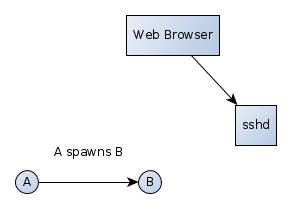
\includegraphics[scale=0.5]{images/client-arcitechure.png}
%\caption{A View of Client Architecture}
%\end{figure}
%
%The client's job is to find the server and provide a way for the server to connect with the client.